\section{Učenje}

Namen naloge je generirati, naučiti in testirati nevronsko mrežo za prepoznavanje ročno napisanih števk. S pomočjo modula \texttt{pyTorch} sem generiral nevronsko mrežo s 3 sloji. Prvi, vhodni ima dimenzijo 28x28 = 784 in izhodni 10, kar predstavlja števke od 0 do 9, za srednjo, nevidno plast, lahko izbiram poljubno velikost. Za učenje sem uporabil podatke iz \href{https://yann.lecun.com/exdb/mnist/}{MNIST baze}, ki vsebuje 60 000 slik s pripadajočimi oznakami za učenje in 10 000 testnih slik z rešitvami. Del baze za učenje je prikazan na sliki \ref{fig:data}, porazdelitev po števkah pa na \ref{fig:data_hist}.

Nevronsko mrežo z velikosjo nevidne plasti 256 sem naučil na 60 000 podatkih v več epohah, kjer sem najprej izračunal odgovor mreže na sliko v tako zvanem ``forward pass'', nato glede na dobljen odgovor mreže in znano rešitev določil skupno napako. Sledi ``backward pass'' in posodobitev uteži, glede na definirano hitrost učenja $Lr$, za kar sem uporabil optimizatorje v \texttt{torch.optim} SGD in ADAM.

Kot je razvidno na sliki \ref{fig:learn_curve} oba delujeta različno. SGD (Stohastic Gradient Descend), je preprostejši in hitrejši, vendar potrebuje razmeroma višjo hitrost učenja, dočim je metoda ADAM (Adaptive Moment Estimation) računsko zahtevnejša in terja nižje hitrosti učenja, prav tako pa  potrebuje manj epoh.

Ugotovil sem, da je za klasifikacijske probleme najboljša ocena skupne napake z \\\texttt{torch.nn.CrossEntropyLoss} s povprečenjem
\begin{align}
    \ell(x, y) =& \sum_{n=1}^{N} \frac{l_n}{\sum_{n=1}^{N}\, w_{y_n}} , \\\nonumber
    l_n =& - w_{y_n} \log \left( \frac{\exp(x_{n, y_n})}{\sum_{c=1}^{C} \exp(x_{n,c})} \right),
\end{align}
kjer je $x$ vhod in $y$ izhod, $w$ utež, $N=6 \cdot 10^4$ dimenzija problema in $C=28\cdot28$ velikost vhoda. Pri tem izhodna plast dimenzije 10 predstavlja tudi dejanske vrednosti števk.

Prav tako lagko iz slike \ref{fig:learn_curve} sklepam, da je za SDG optimizator najprimerneje izbrati hitrost učenja 0.1 in 20 epoh, saj nato skupna napaka rahlo divergira. Tam je točnost modela 97.9\% in skupna napaka 0.0677. ADAM se še najbolje obnese pri $Lr=0.001$ in 10 epoh, kjer doseže točnost 98.0\% in vrednosti skupne napake 0.0745, verjetno bi moral poskusiti še z nižjimi hitrostmi učenja.

\begin{figure}[H]
    \centering
    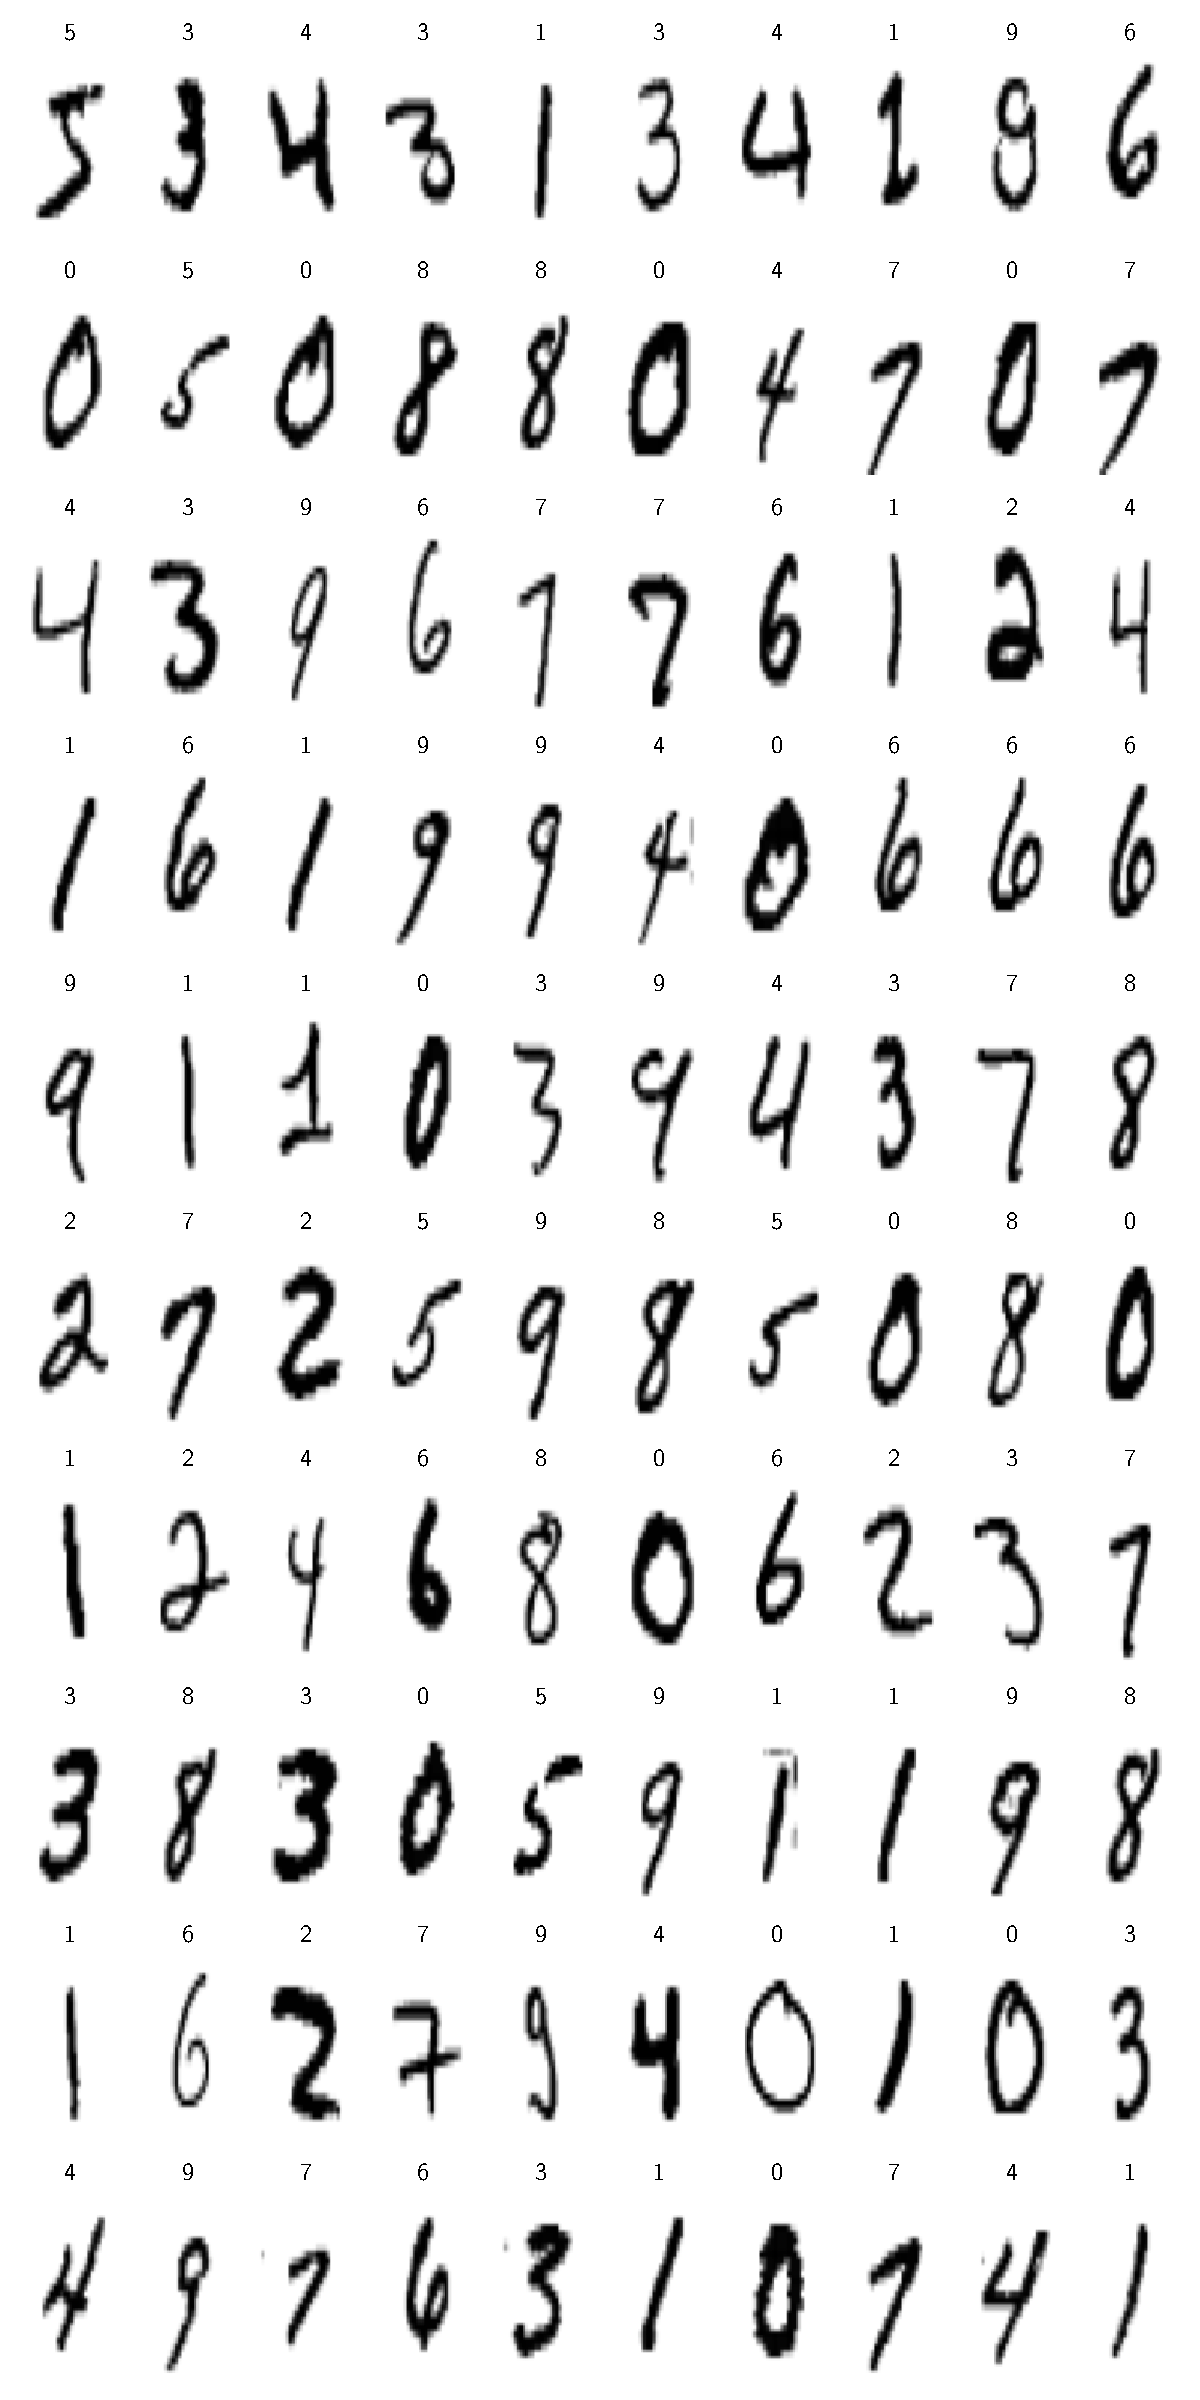
\includegraphics[height=23cm]{13.nal_slike/train_images.pdf}
    \caption{Podatki: 60 000 slik 28x28 px}\label{fig:data}
\end{figure}

\begin{figure}[H]
    \centering
    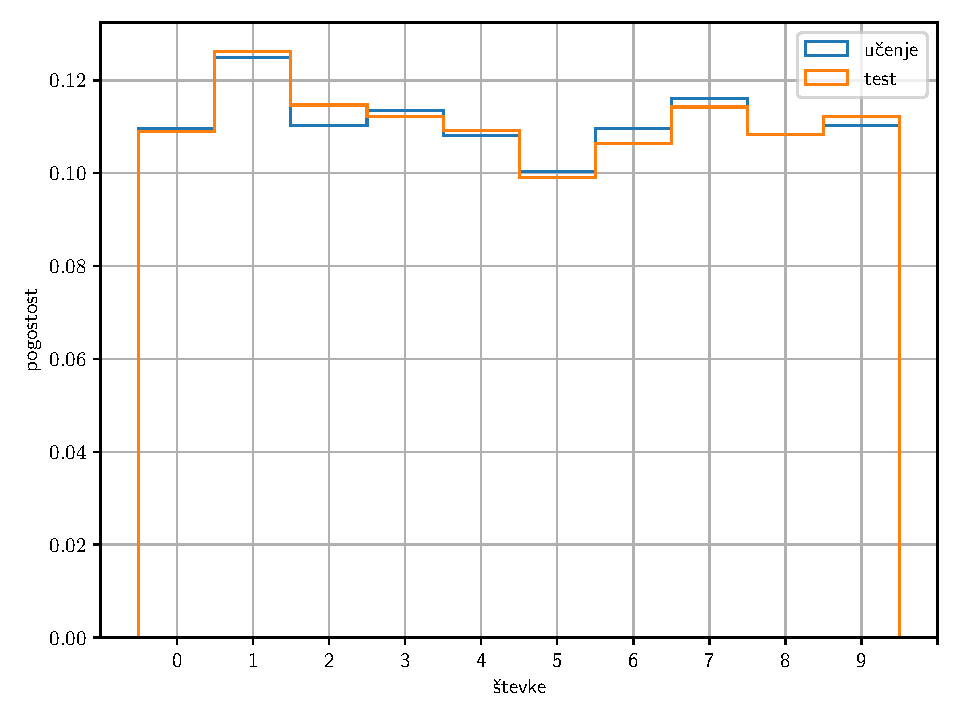
\includegraphics[width=0.6\textwidth]{13.nal_slike/MNIST_hist.pdf}
    \caption{Porazdelitev števk po bazah podatkov}\label{fig:data_hist}
\end{figure}

\begin{figure}[H]
    \centering
    \begin{subfigure}{0.7\textwidth}
        \centering
        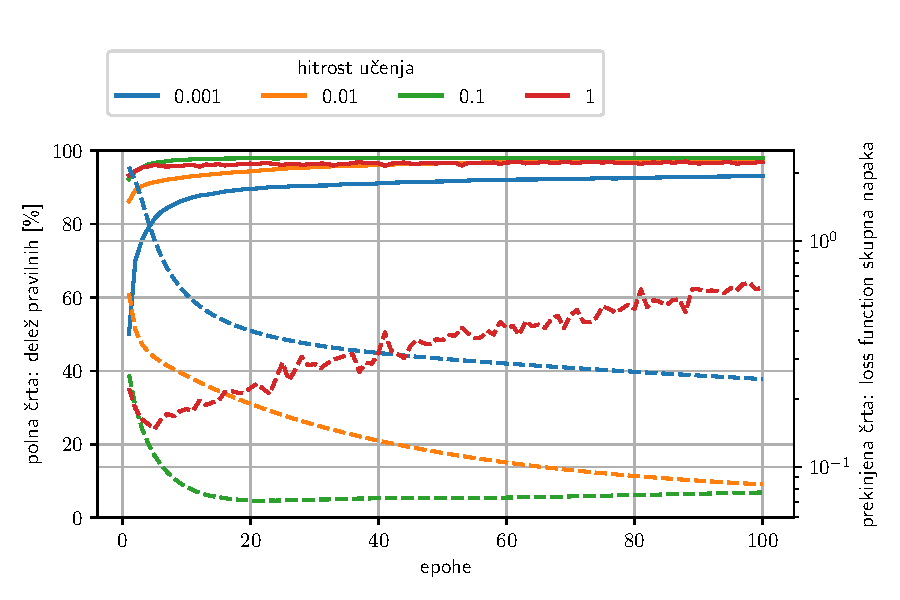
\includegraphics[width=\textwidth]{13.nal_slike/learning_curve_SDG.pdf}
        \caption{SGD}
    \end{subfigure}
    \begin{subfigure}{0.7\textwidth}
        \centering
        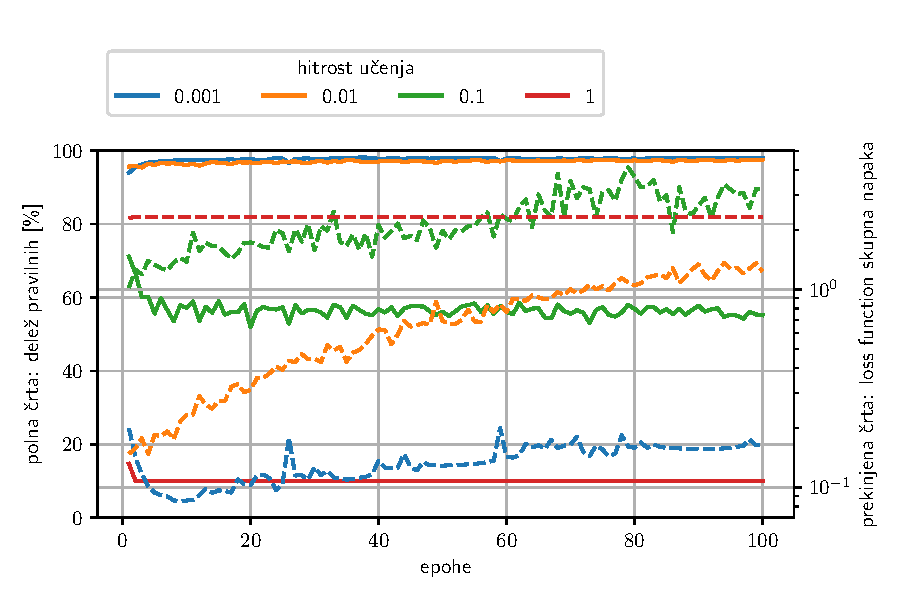
\includegraphics[width=\textwidth]{13.nal_slike/learning_curve_ADAM.pdf}
        \caption{ADAM}
    \end{subfigure}
    \caption{Krivulja učenja za različne hitrosti in minimizatorja skupne napake}\label{fig:learn_curve}
\end{figure}

Preverim tudi, kako vmesna plast vpliva na točnost učenja in opazim, da točnost močno pade za zelo majhno skrito plast (manjša od izhodne), kar je pričakovano. V obratnem primeru pa se točnost bistveno ne izboljša, sploh nad cca. 100-200 je izboljšava minimalna, zato bom za vse nadaljne izračune uporabljal 3-plastno mrežo z 256 nevroni na skriti plasti.

\begin{figure}[H]
    \centering
    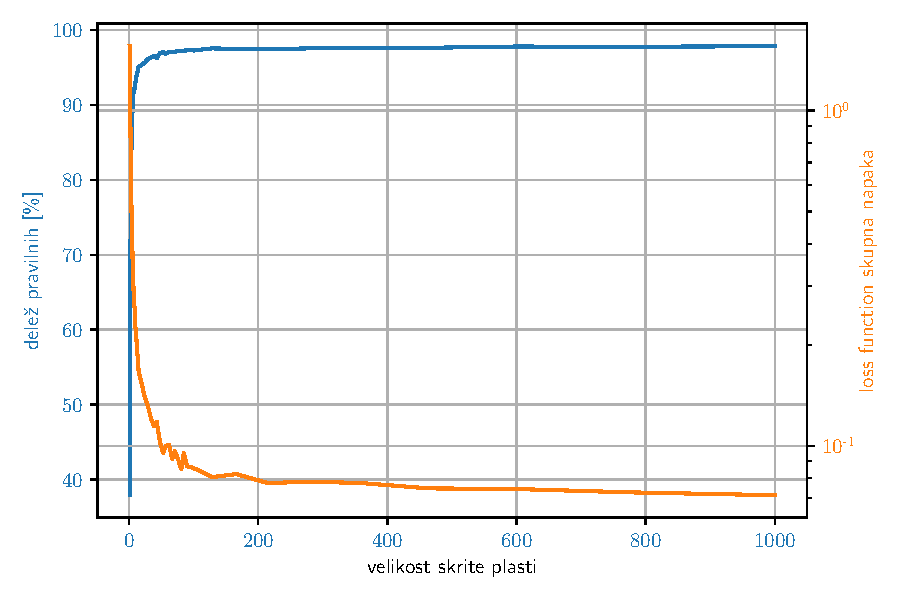
\includegraphics[width=0.55\linewidth]{13.nal_slike/velikost_skrite_plasi.pdf}
    \caption{Vpliv velikosti skrite plasti}
\end{figure}

\subsection{Več skritih plasti}

Poskusimo tudi modele z več vmesnih plasti, pri čemer sem definiral upad velikosti linearno med vhodom (28x28=784) in izhodom(10)
\begin{equation}
    H = \frac{784-10}{N+1},
\end{equation}
kjer je $N$ število skritih plasti. Predvsem opazim, da dodatne plasti očitno povečajo računski čas, za izboljšave bi verjetno potreboval bolje nastaviti parametre učenja (hitrost, epohe), saj izboljšanja ni opaziti iz izračunov, prikazani na spodnji sliki, kjer sem uporabil SGD optimizator, $Lr=0.001$ in 20 epoh. Pri krivulji učenja je tudi opaziti nekaj oscilacij, kar po mojem mnenju ni najbolj `zdravo', zato raje računam s klasično 3-plastno mrežo, opisano poprej.

\begin{figure}[H]
    \centering
    \begin{subfigure}{0.49\textwidth}
        \centering
        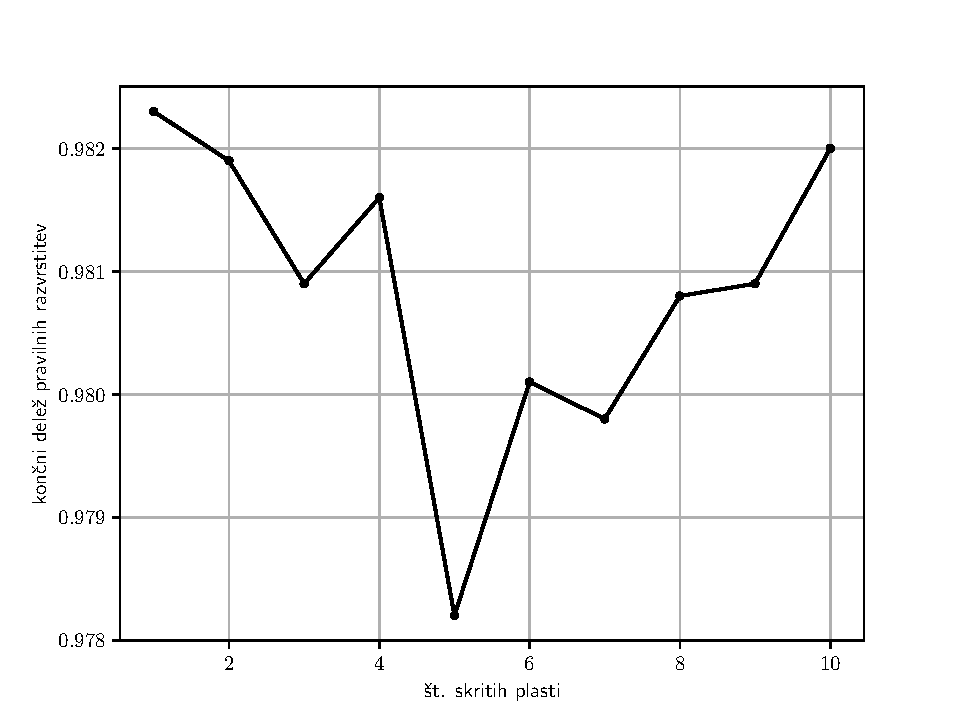
\includegraphics[width=\textwidth]{13.nal_slike/vec_plasti_koncno.pdf}
        \caption{končna točnost}
    \end{subfigure}
    \begin{subfigure}{0.49\textwidth}
        \centering
        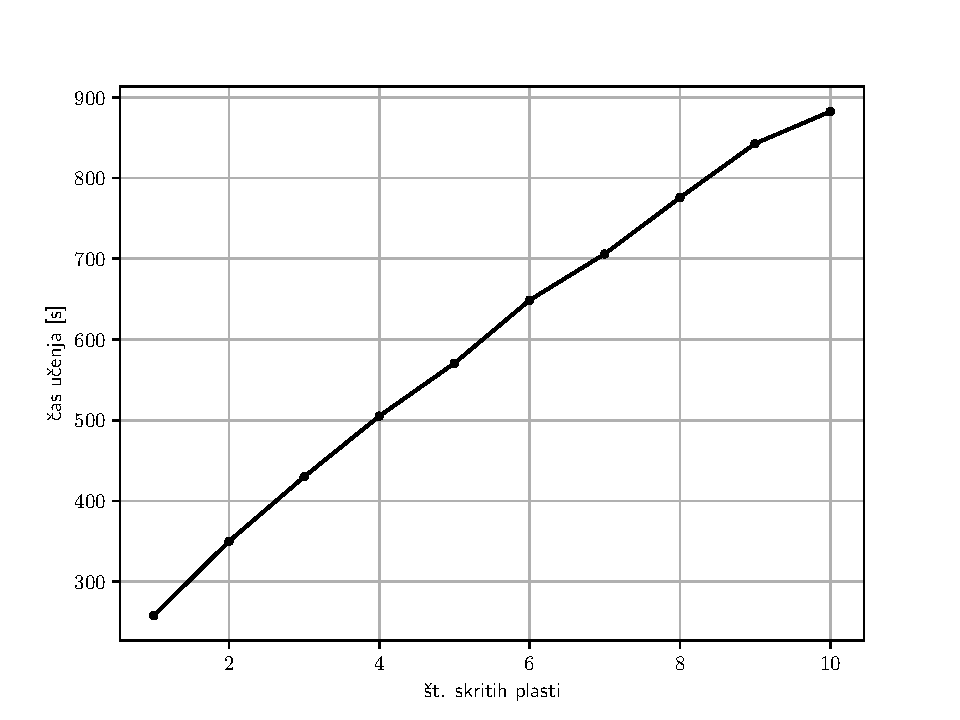
\includegraphics[width=\textwidth]{13.nal_slike/vec_plasti_time.pdf}
        \caption{računski čas}
    \end{subfigure}
    \caption{Učenje mreže z več vmesnimi plastmi}
\end{figure}

\subsection{Konvolucijska mreža}

Izdelal sem tudi mrežo z dvoje konvolucijskimi in dvoje linernimi plastmi za določanje števk. Prva plast je 2D konvolucijska z enim vhodom (28x28 slika) in 32 izhodi, druge pa ima 32  vhodov in 64 izhodov. Te sem nato peljel preko dveh linernih plasti na 128 in nato na 10 izhodov, kot je število števk. Mrežo sem naučil z optimizatorjem SGD v 10 epohah s hitrostjo učenja 0.1, kar je prikazano na spodnji sliki.

Rezultat je malenkost boljši od prejšnjih, vendar bi ga verjetno lahko z bolj finimi nastavitvami še bolj izboljšal, dočim je to pri linernem modelu težje.

\begin{figure}[ht]
    \centering
    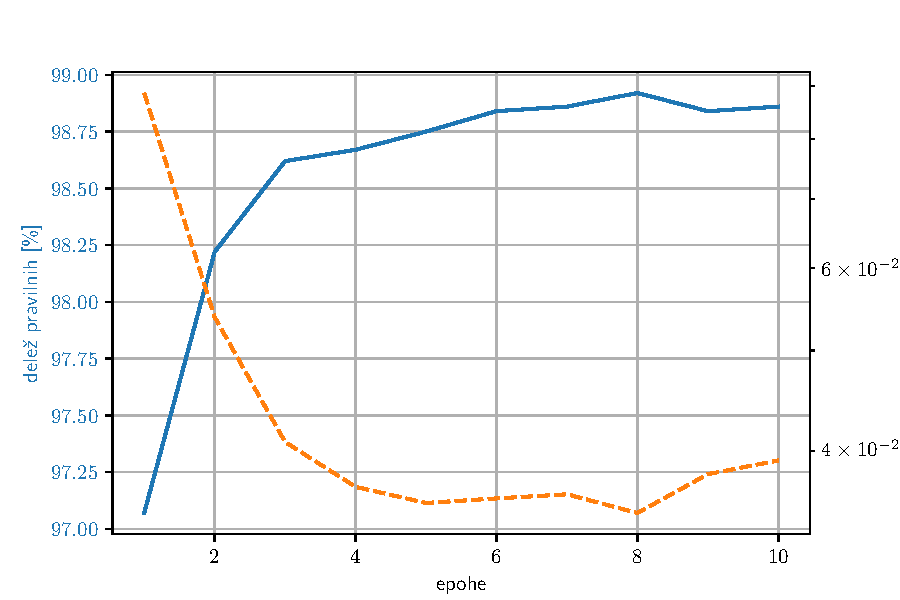
\includegraphics[width=0.55\linewidth]{13.nal_slike/konvolucijska.pdf}
    \caption{Konvolucijska nevronska mreža}
\end{figure}

\begin{table}[ht]
    \centering
    \begin{tabular}[ht]{c||c|c|c}
        model & SGD linear & ADAM linear & konvolucijska mreža \\\hline\hline
        točnost & 97,9 & 98,0 & 98,9 \\\hline
        skupna napaka & 0,0677 & 0,0745 & 0,0392 \\\hline
    \end{tabular}
    \caption{Primerjava točnosti modelov}
\end{table}

\section{Testiranje}

Poglejmo, katere števke je model linearne mreže s SGD optimizatorjem določil napačno. Na spodnji sliki je prikazano nakaj primerov, vsem pa je skupno, da je bila odločitev precej tesna, v nekaterih primerih pa je žal prevladal napačen izhod. Povečini pa je pravilen izhod tudi precej vidoko utežen, kar nakazuje na pravilno delovanje algoritma! Rdeče obarvane so napovedi mreže, zeleno pa prave števke.

\begin{figure}[ht]
    \centering
    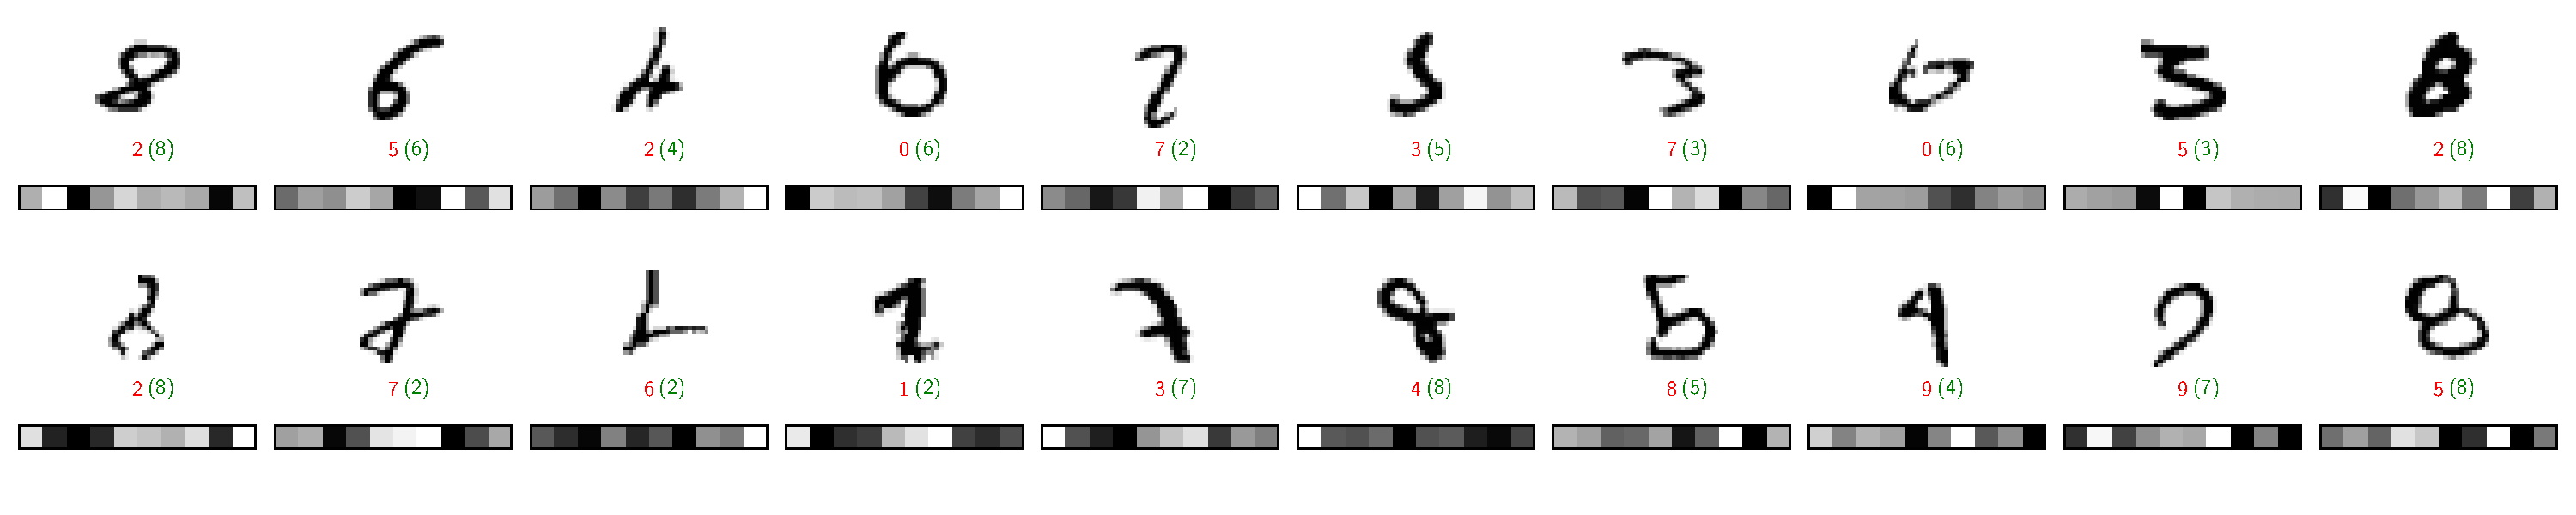
\includegraphics[width=\linewidth]{13.nal_slike/napake_ADAM.pdf}
    \caption{Napačno razvrščene števke}
\end{figure}

Sledi podrobnejši prikaz, katere števke algoritem zamenjuje. Kot prvo je opazna očitna razlika med vsemi modeli, očitno učenje (in optimizator) odločilno vpliva na rezultat. Na testeni paket 10 000 slik sem spustil naučeno mrežo in preverjal pravilnost izračuna. Ob napaki sem shranil izračunano in pravilno števko ter na njeno mesto v matriki zamenjav prištel 1. Na spodnjih slikah so prikazane te matrike zamenjav.

Opazim, da s SGD naučen model najpogosteje zamenjuje 7 za 2 ali 9, 9 za 4 , 4 za 9 in 6 za 5. Pri ADAM prevladuje predvsem zamenjava 5 za 3, pri konvolucijski pa 7 za 2.

Nekatere zamenjave so zaradi podobnosti števk (2 in 7, 3 in 5, 5 in 6...) upravičene in bi jih zaradi slabšega poznavanja ameriškega zapisa storil tudi sam.

Prikazan je tudi histogram porazdelitve izračunaih in pričakovanih vrednosti, ki potrjuje zgornje ugotovitve iz matrik zamenjav.

\begin{figure}[H]
    \centering
    \begin{subfigure}{0.75\textwidth}
        \centering
        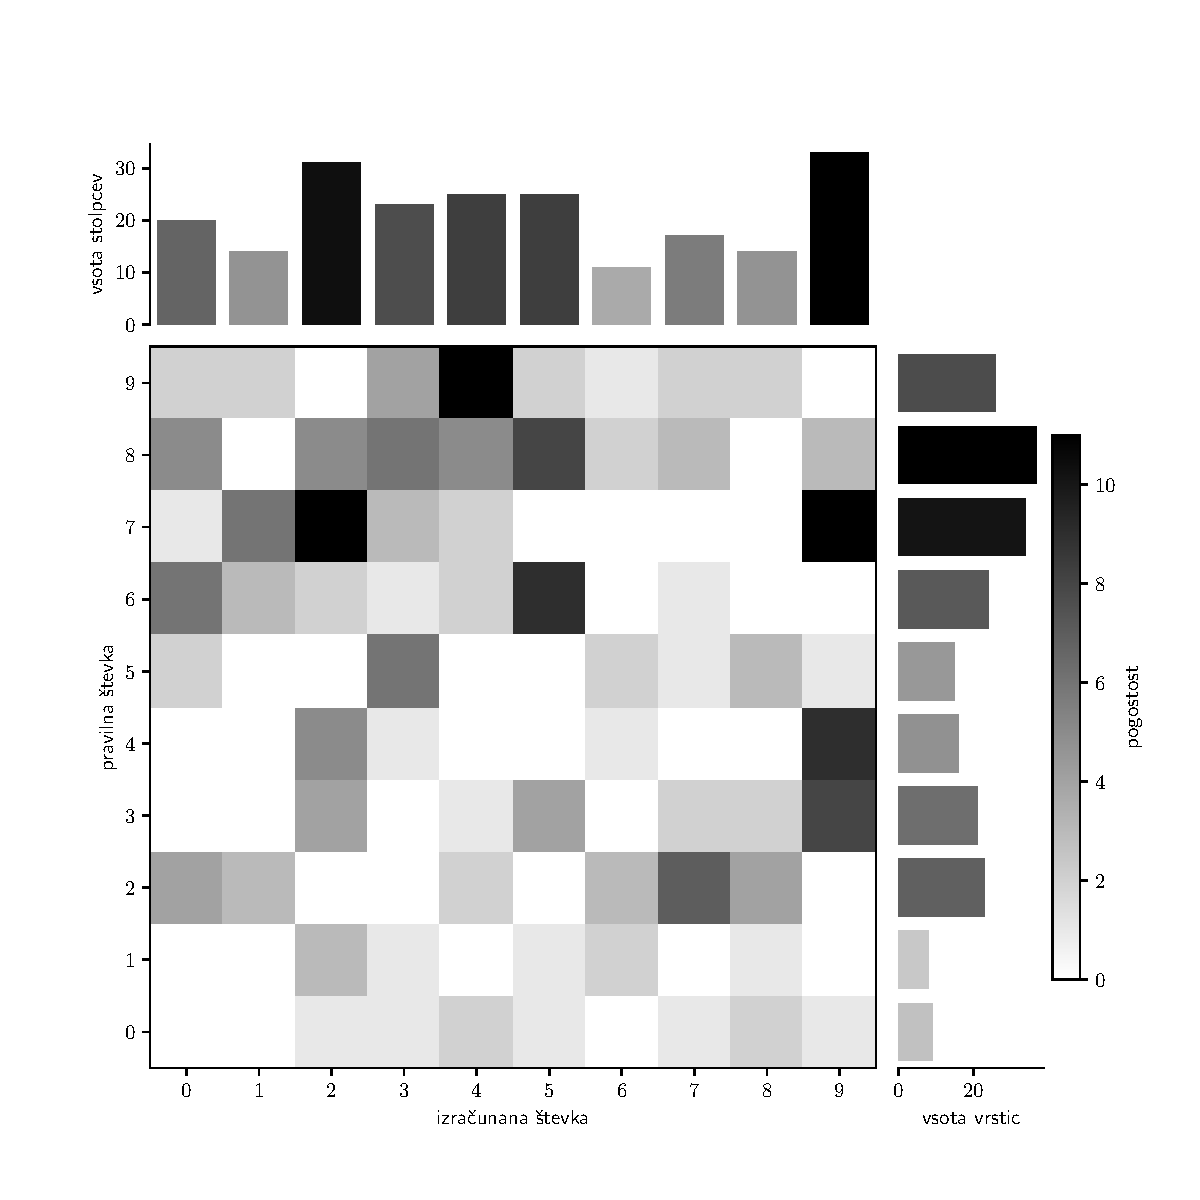
\includegraphics[width=\textwidth]{13.nal_slike/zamenjave_SDG.pdf}
        \caption{SGD}
    \end{subfigure}
    \begin{subfigure}{0.75\textwidth}
        \centering
        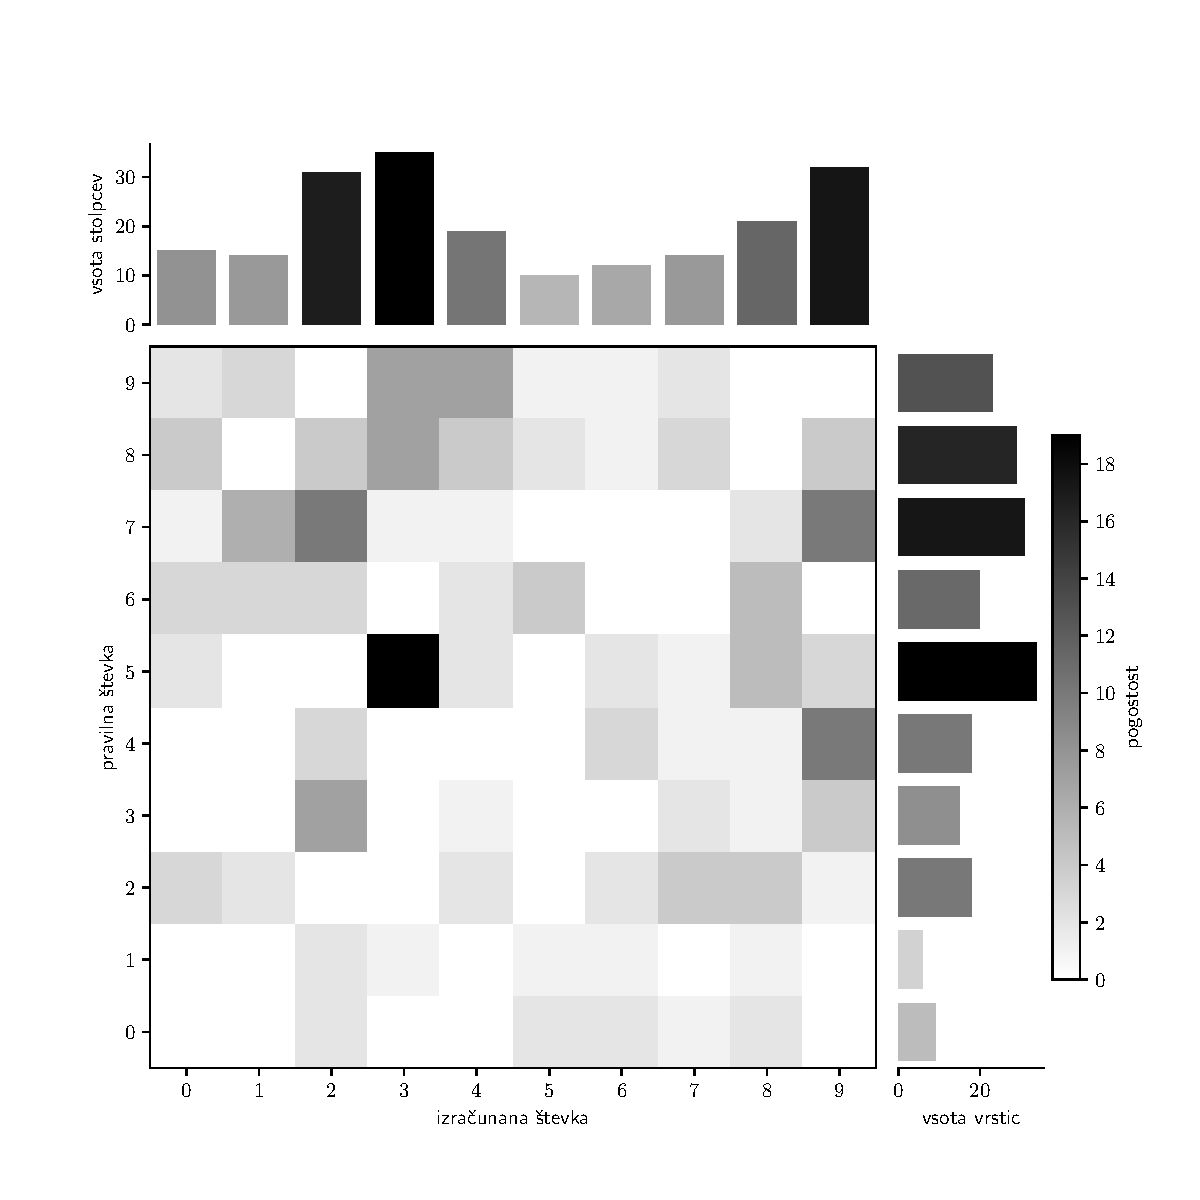
\includegraphics[width=\textwidth]{13.nal_slike/zamenjave_ADAM.pdf}
        \caption{ADAM}
    \end{subfigure}
    \caption{Matrika zamenjav}
\end{figure}

\begin{figure}[ht]
    \centering
    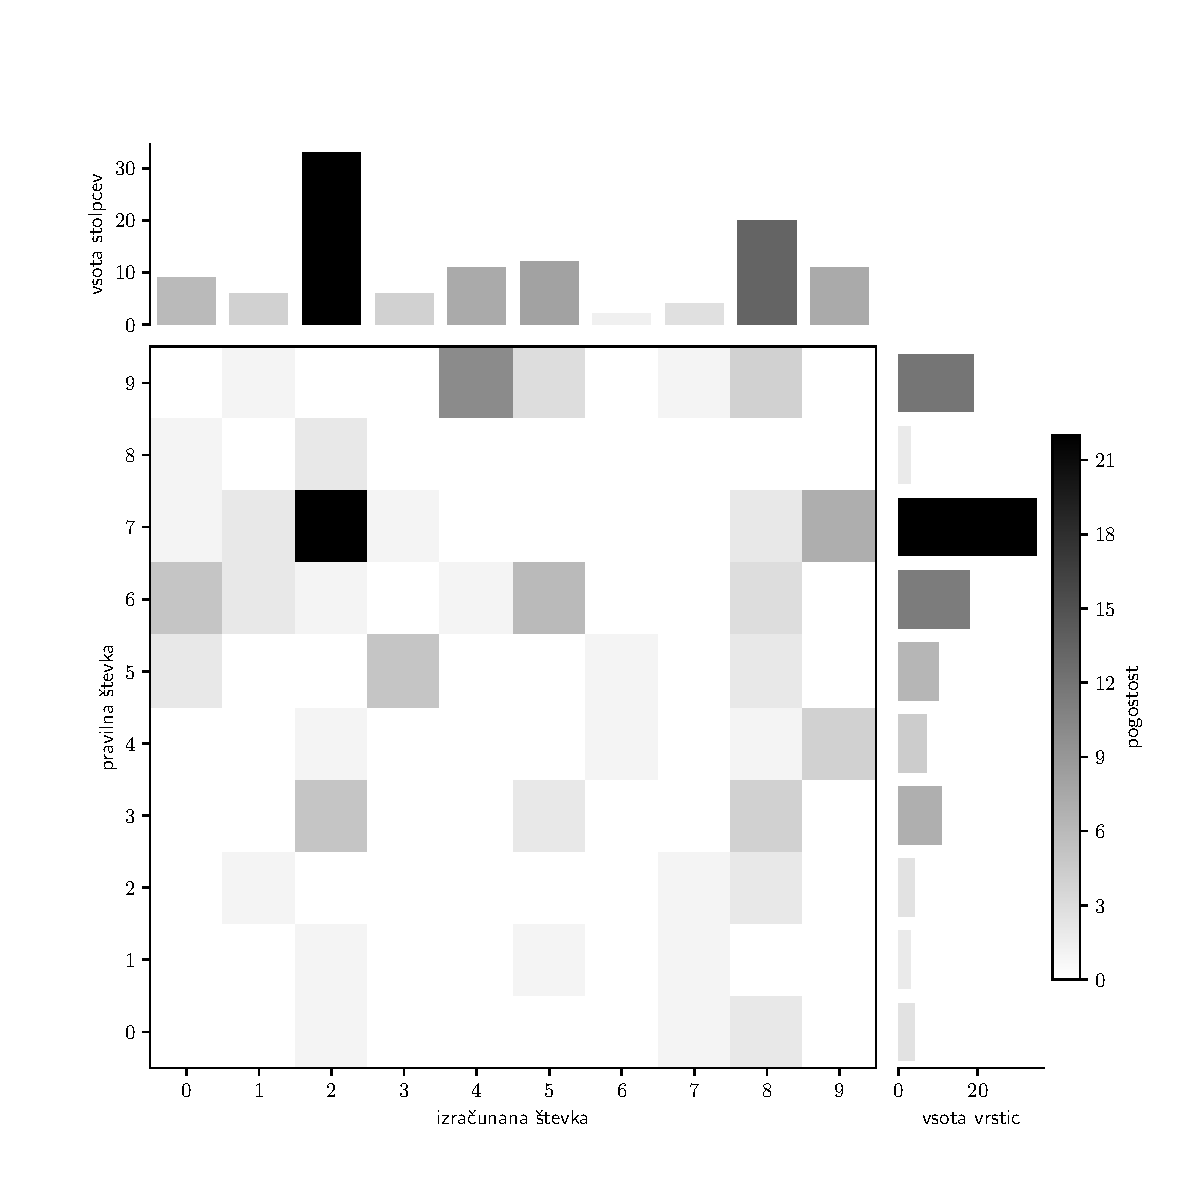
\includegraphics[width=0.75\textwidth]{13.nal_slike/zamenjave_konv.pdf}
    \caption{Matrika zamenjav, konvolucijska mreža}
\end{figure}

\begin{figure}[ht!]
    \centering
    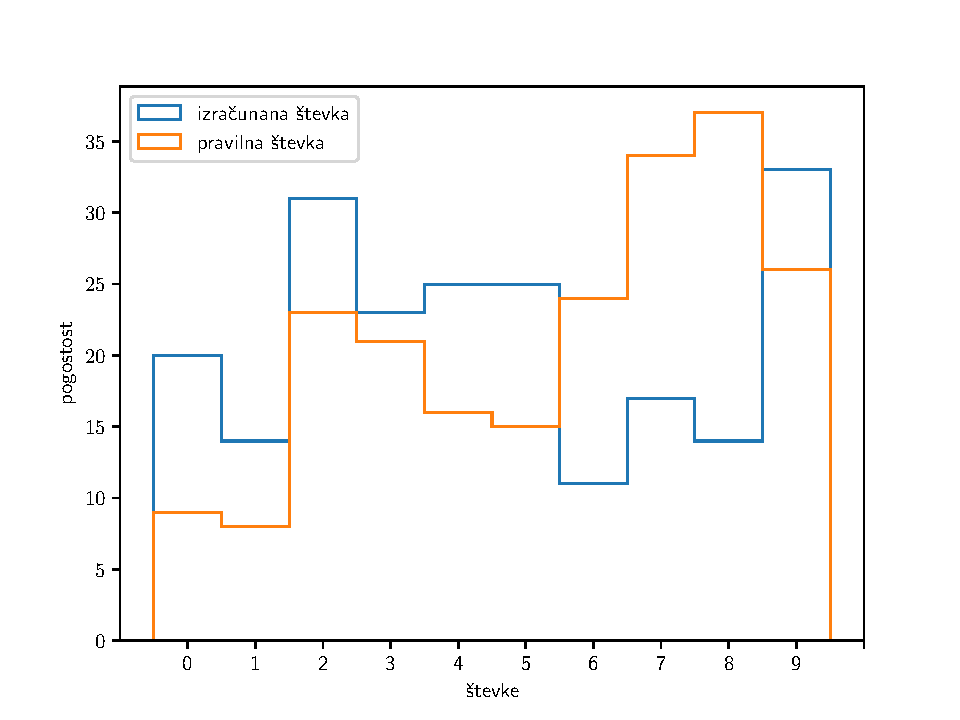
\includegraphics[width=0.6\linewidth]{13.nal_slike/zamenjave_SDG_hist.pdf}
    \caption{Histogram napačnih izračunov z SGD modelom}
\end{figure}

\subsection{Vplivi na odločitev mreže}

Na rezultat mreže vpliva več dejavnikov, med drugim že sam proces učenja, nato pa kombinacija zasnove mreže in uteži ter vhodni podatki sami. V tem pod-poglavju bom analiziral vpliv vhodnih podatkov na odločitev mreže.

To sem izračunal tako, da sem vzel vhodno sliko in pričakovan izhod zanjo (pravilna rešitev). Na podlagi napake (na slikah loss) med napovedjo mreže iz danega vhoda in pričkavanim (idealnim) izhodom sem izračunal odvode (gradiente) vhodne slike z \\\texttt{torch.autograd.grad}, pri čemer sem za izhode odvajane funkcije vzel izračunane napake. Tako dobljene odvode na vhodi sliki je potrebno le še skalirati na interval (0,1) in prikazati na spodnji sliki.

Opazim, da na odločitev sploh ne vplivajo najbolj obarvani piksli. Najbolj zanimivo je, da na odločitev med podobnimi si števili najbolj vplivajo detajli, kot je npr. `uho' na petici, ki jo loči od devetice, predvsem pri linernih modelih. Zanimivo, da tega za SGD optimizator med 5 in 6 ni tako izrazito opaziti, zato je verjetno to vzrok, da algoritem zamenjuje ti števki pogosteje. Tudi med npr. 1 in 7 ni opaziti zaznave očitne razlike - strešice.

Razlogov za (edini) očitni zamenjavi konvolucijske in linerane ADAM mreže iz spodnjih slik ni tako enostavno izluščiti. Za razliko med 2 in 7 pri konvolucijski mreži bi bilo verjetno potrebno bolje zaznati `repek', verjetno pa algoritem motijo rotacije števil. Za bolj natančne analize bi moral povprečiti več napačnih odločitev in jih primerjati z pravimi.

\begin{figure}[ht!]
    \centering
    \begin{subfigure}{\textwidth}
        \centering
        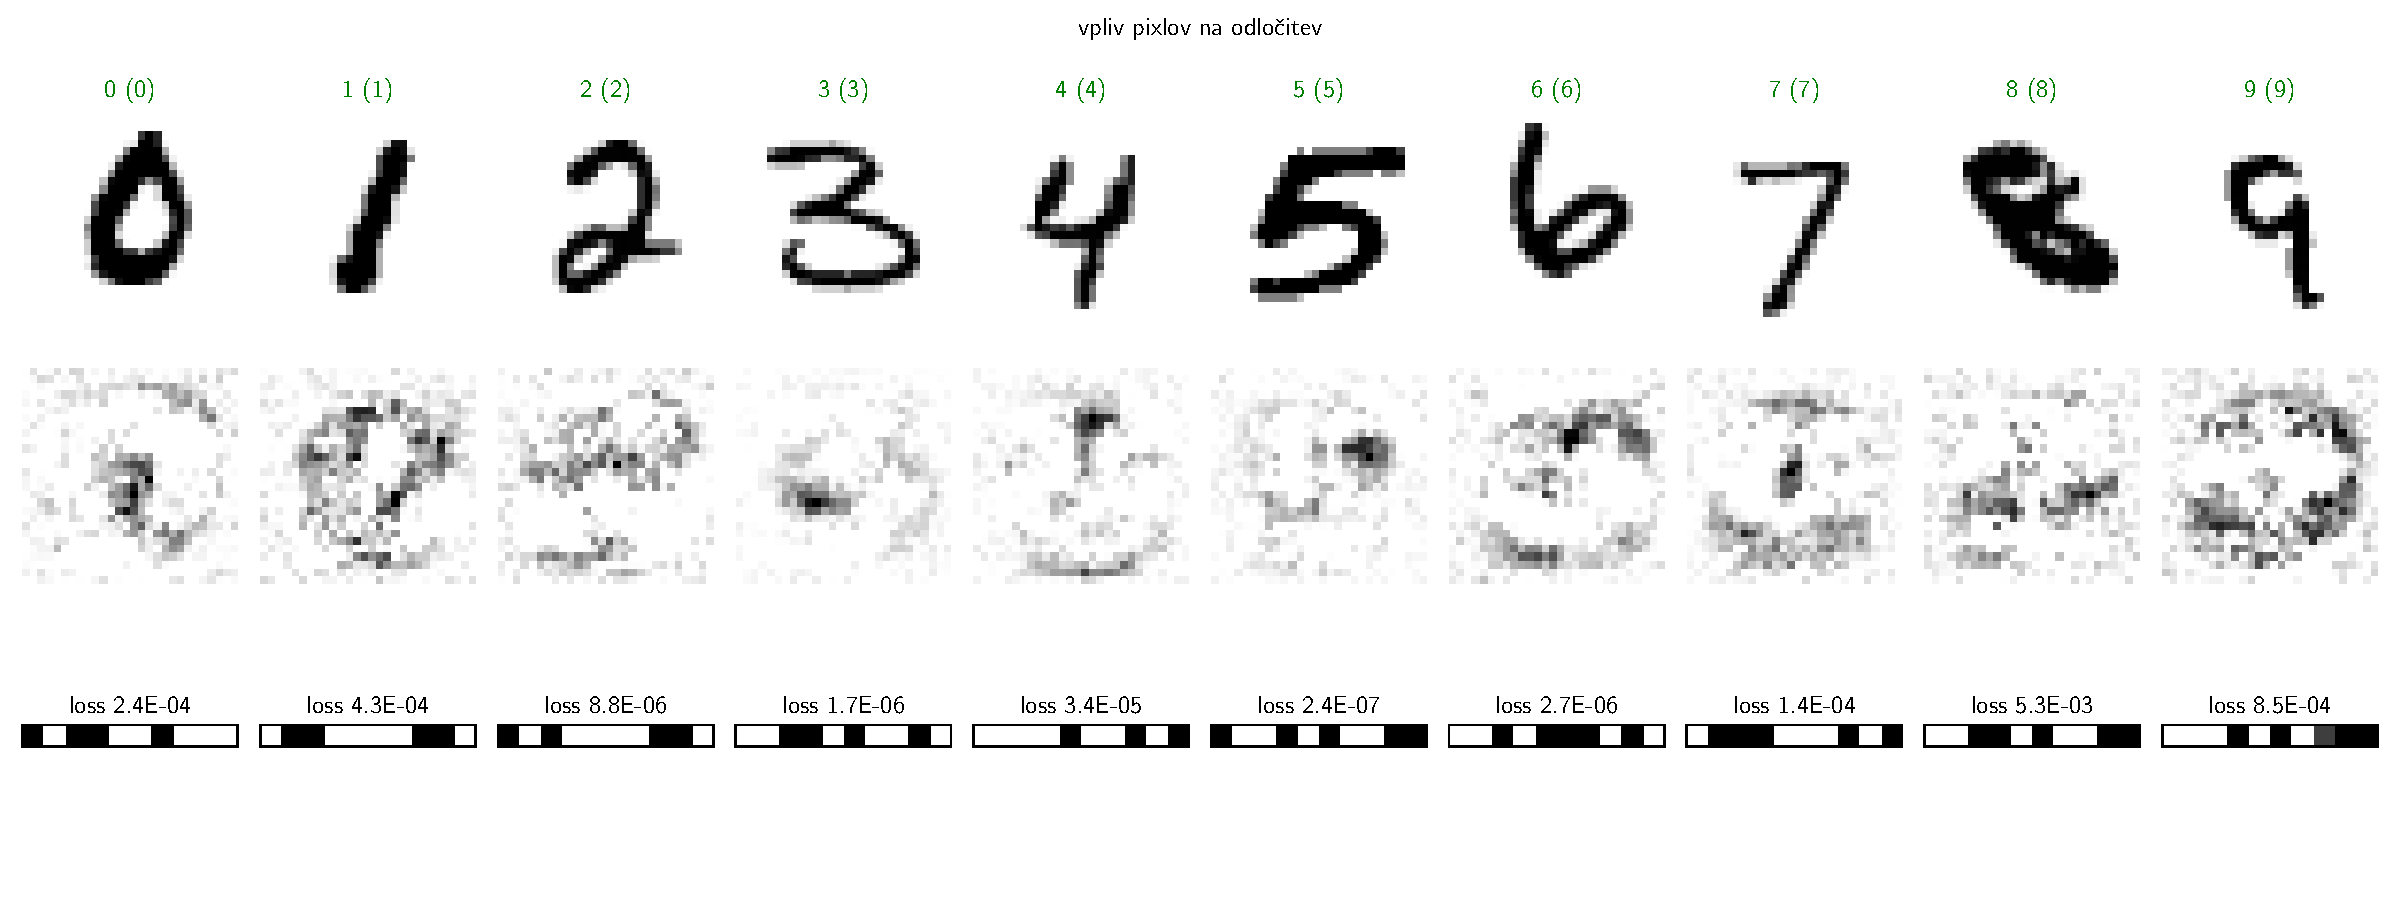
\includegraphics[width=\linewidth]{13.nal_slike/vpliv_px_SGD.pdf}
        \caption{Linearna mreža SGD}
    \end{subfigure}
    \begin{subfigure}{\textwidth}
        \centering
        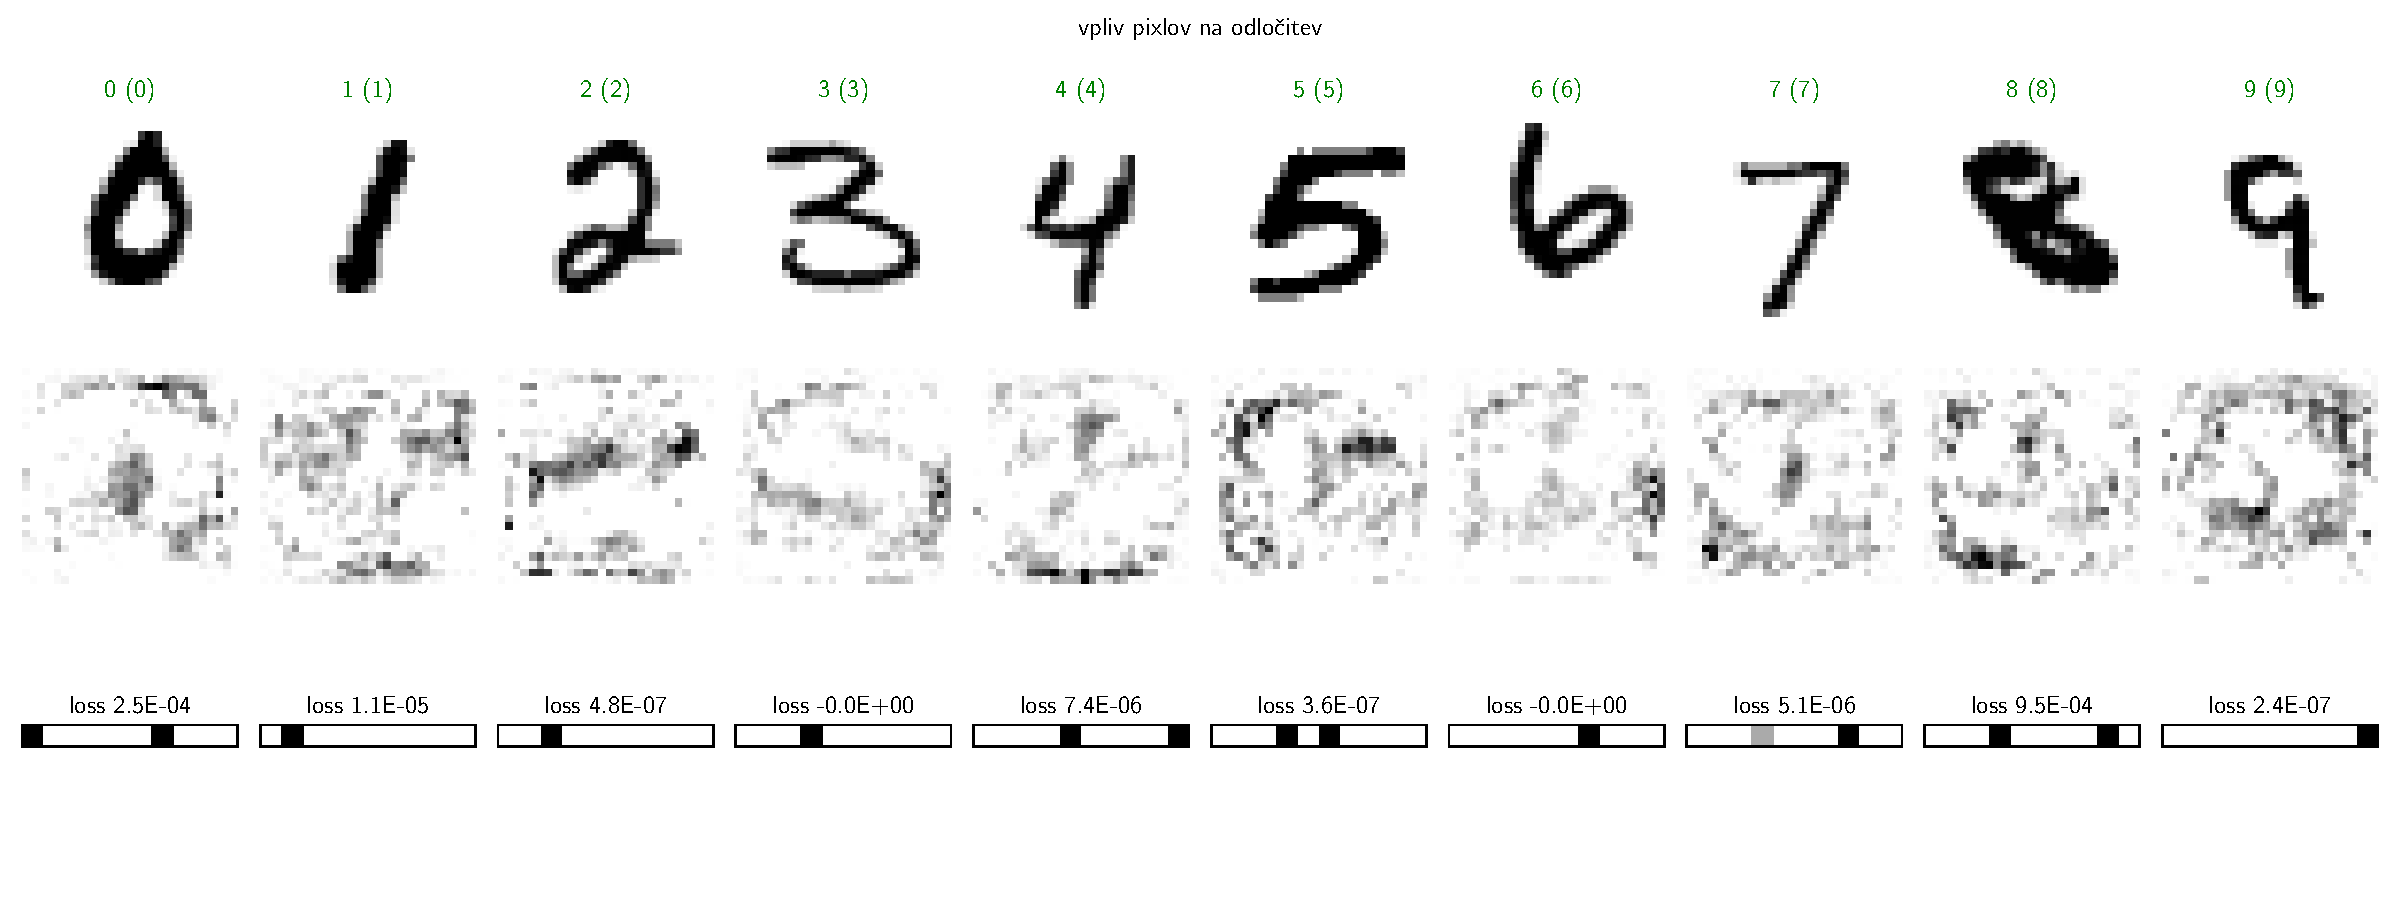
\includegraphics[width=\linewidth]{13.nal_slike/vpliv_px_ADAM.pdf}
        \caption{Linearna mreža ADAM}
    \end{subfigure}
    \begin{subfigure}{\textwidth}
        \centering
        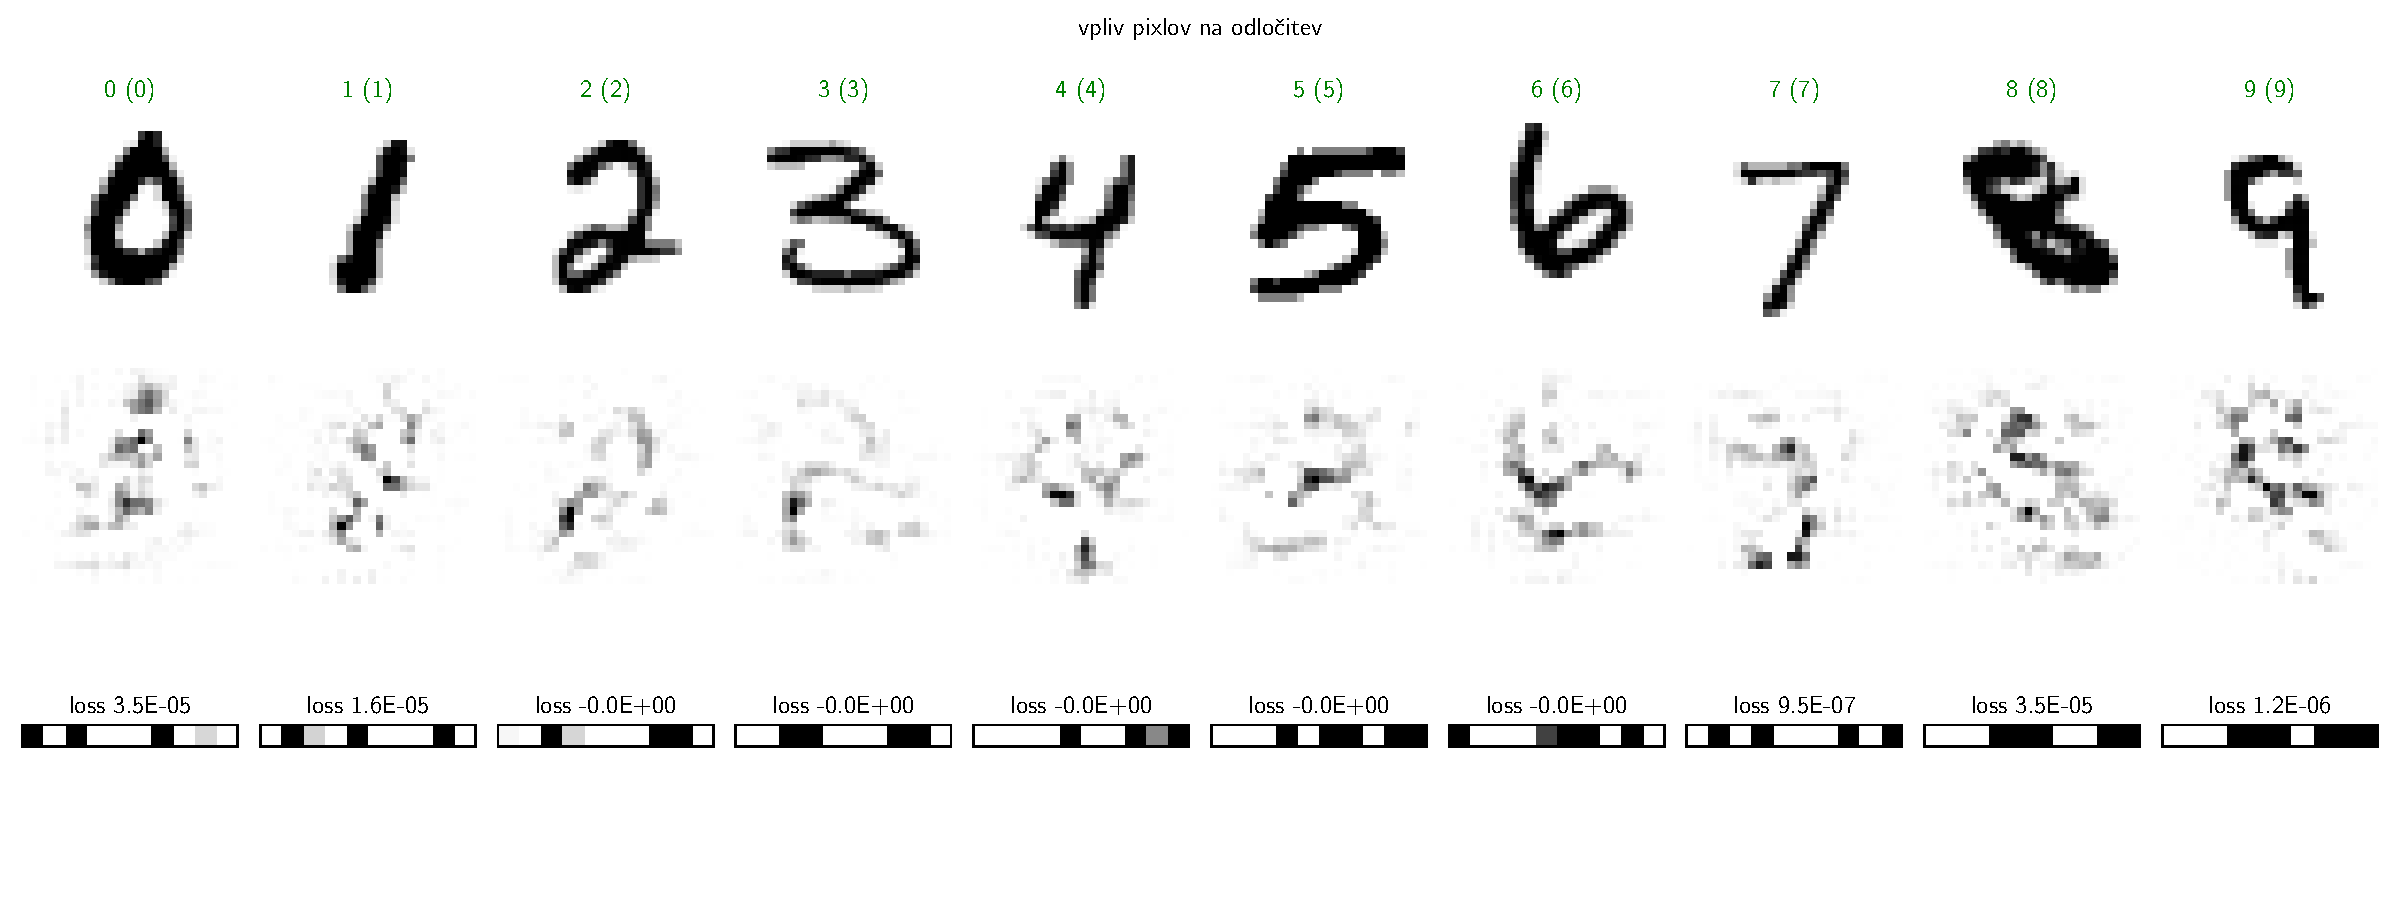
\includegraphics[width=\linewidth]{13.nal_slike/vpliv_px_konv.pdf}
        \caption{Konvolucijska mreža}
    \end{subfigure}
    \caption{Pomembnost pikslov pri odločanju mreže}
\end{figure}

Poleg tega lahko opazim tudi, da so odločitve precej tesne, pogosto je podobnih vrednosti večje število izhodnih nevronov, edino linearna ADAM mreža se izkaže bolje, in v nekaterih primerih vrne celo idealen izhod. Za preostali dve bi moral preveriti več odzivov za enako števko.

\subsection{Naključni podatki}

Genreirial sem še 10 000 slik z naključnimi podatki, enakomerna na intervalu (0,1) in z Gaussovo porazdelitvijo s $\sigma = \mu = 1$, skalirano na interval (0,1). Očitno se mreža težko odloči, saj je izhod precej nejasen. Očitno je le, da nekatere števke pogosteje zazana, naktere pa nikoli! To velja za vse tri modele brez bistvenih razlik, zato prikažem le za enega.

Pričakoval sem sicer bolj uravnovešene rezultate zato tega ne znam prav dobro pojasniti. Zanimivo bi bilo tudi, če bi šum dodajal slikam iz MNIST baze, vendar puščam to za drugič.

\begin{figure}[ht]
    \centering
    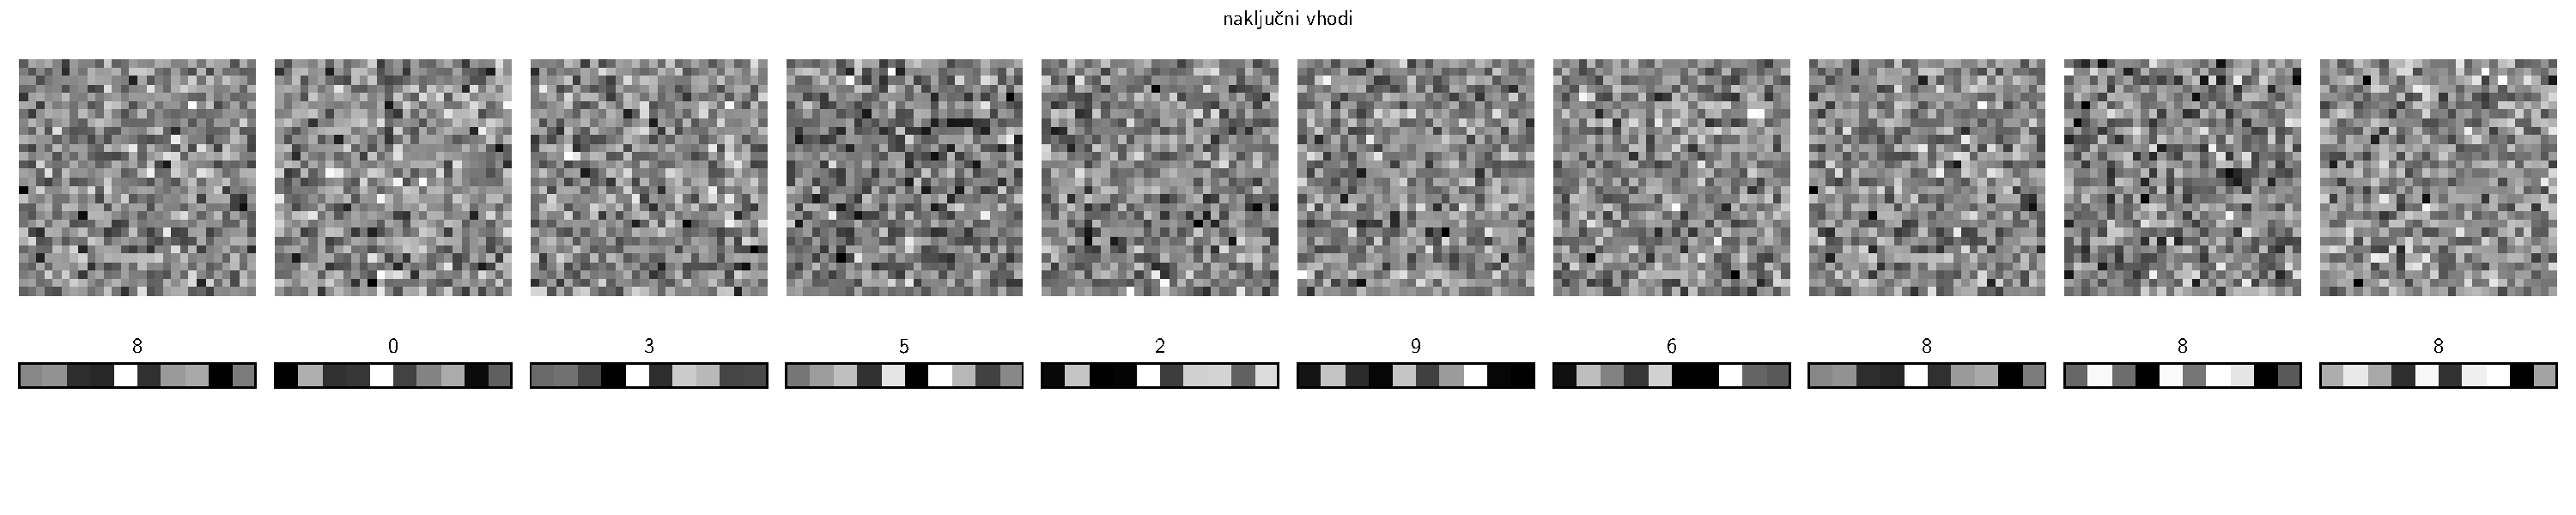
\includegraphics[width=\linewidth]{13.nal_slike/naklj_data_gauss.pdf}
    \caption{Razvrščanje naključnih podatkov z Gaussvo porazdelitvijo}
\end{figure}

\begin{figure}[ht]
    \centering
    \begin{subfigure}{0.49\textwidth}
        \centering
        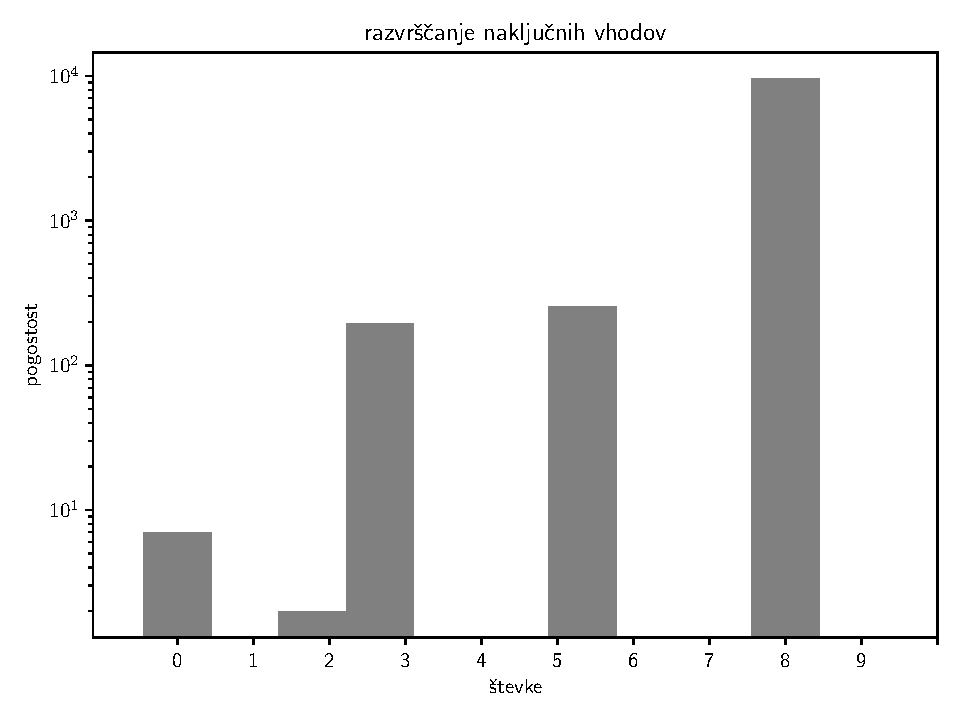
\includegraphics[width=\textwidth]{13.nal_slike/naklj_data_hist.pdf}
        \caption{enakomerno na intervalu (0,1)}
    \end{subfigure}
    \begin{subfigure}{0.49\textwidth}
        \centering
        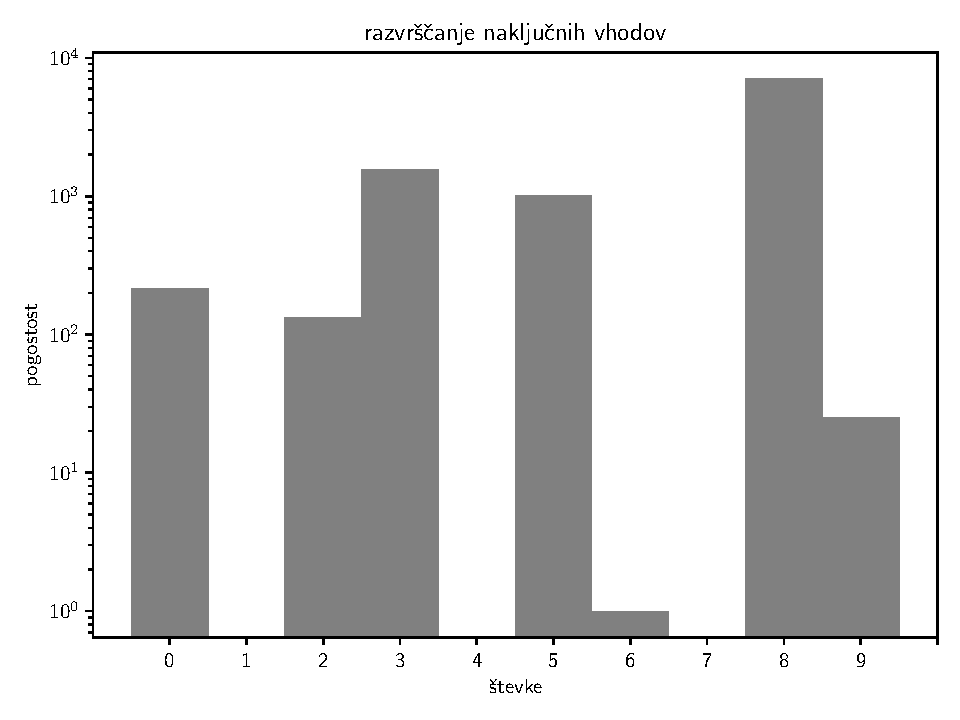
\includegraphics[width=\textwidth]{13.nal_slike/naklj_data_gauss_hist.pdf}
        \caption{Gaussova porazdelitev}
    \end{subfigure}
    \caption{Razvrščanje naključnih podatkov}
\end{figure}

\section{Deep dream}

Na že naučeni mreži sem preveril, kaj mreža `pojmuje' kot idealne števke. To sem storil na podoben način, kot sem učil mrežo, vendar brez posodobitve uteži. Izračunal sem napako med odzivom mreže na nek začetni približek vhoda in idealnim izhodom za neko števko, nato sem izvedel ``backward propagation pass'' in namesto uteži mreže posodobil vhodno sliko. To sem ponavljal v iteracijski zanki do željene napake.

Za začetni približek se še najbolje izkaže matrika ničel, saj v tem primeru v cca. 100 iteracijah že dobimo zadovoljiv vhod z napako (na sliki loss) največ $1\cdot10^{-3}$ pri SGD linearni mreži, pri ADAM in konvolucijski je potrebnih iteracij povečini že nad 1000. Uporabil sem hitrost učenja 0,1 in optimizator SGD.

Predvsem so drugačni rezultati na konvolucijski mreži, kar je pričakovano, glede na popolnoma drugačno zasnovo mreže. Vseeno pa iz sam iz idealnega vhoda mreže težko razberem števke, še najbolj berljive so 0,2 in 3 pri SGD in konvolucijski, ADAM mreža pa ima skoraj popolnoma neberljive podatke.

Pri tem, kot tudi pri pomembnosti pokslov, se vidi predvsem večja primernost konvolucijske mreže za procesiranje slik, saj delujejo piksli tam bolj `urejeno', kot linearna mreža (sploh ADAM).

\begin{figure}[ht]
    \centering
    \begin{subfigure}{\textwidth}
        \centering
        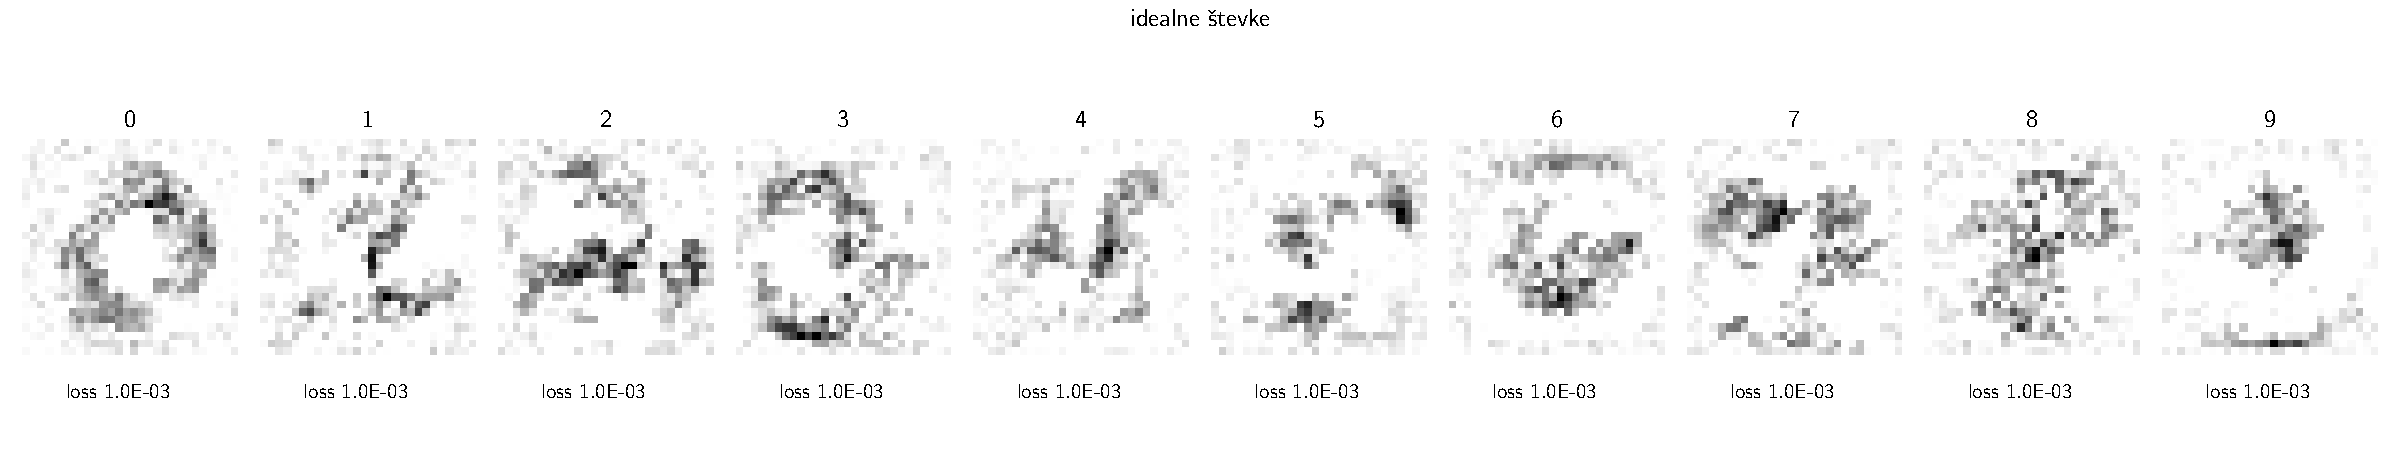
\includegraphics[width=\linewidth]{13.nal_slike/deep_dream_SGD.pdf}
        \caption{SGD}
    \end{subfigure}
    \begin{subfigure}{\textwidth}
        \centering
        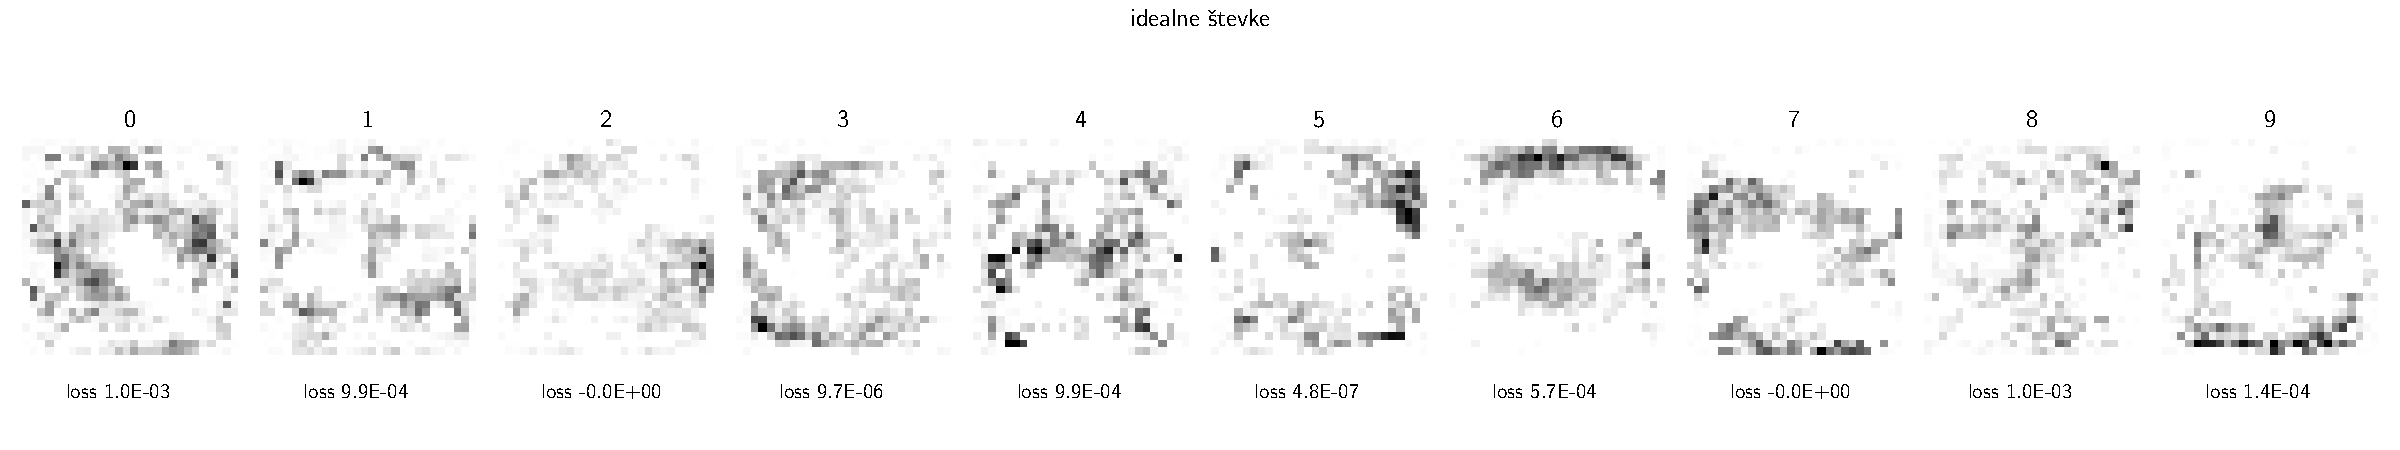
\includegraphics[width=\linewidth]{13.nal_slike/deep_dream_ADAM.pdf}
        \caption{ADAM}
    \end{subfigure}
    \begin{subfigure}{\textwidth}
        \centering
        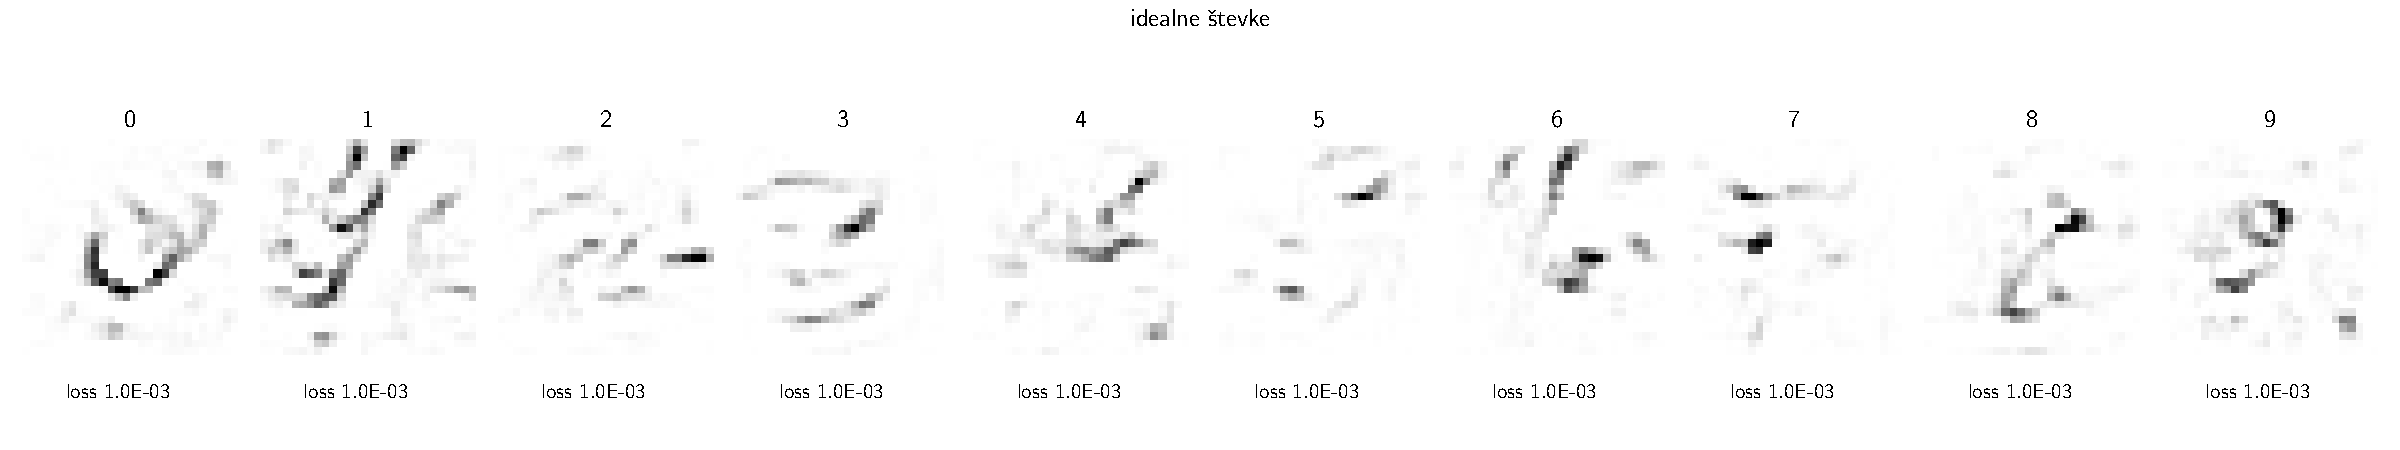
\includegraphics[width=\linewidth]{13.nal_slike/deep_dream_konv.pdf}
        \caption{Konvolucijska}
    \end{subfigure}
    \caption{Deep dream nevronske mreže za števke}
\end{figure}

\section*{Zaključek}

Naloga je bila poučna, sploh po sodobni popularizaciji umetne inteligence. Spoznal sem, da je precej kompleksno predvsem dobro naučiti nevronsko mrežo, pri konvolucijski pa je bilo potrebno še bolj paziti kot pri linearni. Vseeno pa so že rezultati povsem preproste 3-plastne mreže izjemni (nad 95\% točnosti).